%(CHECK Version/Carlo 21.11)\\
%intro was kommt hier?
%\begin{flushleft}
Die von Amazon Web Services(AWS) zu Verfügung gestellte Überwachungswerkzeuge werden in diesem Kapitel vorgestellt. [Rev]Op1{Der Fokus liegt auf Werkzeugen, zur Überwachung von den Kosten oder der Nutzung von AWS-Dienste beitragen.}/Op2{Der Schwerpunkt liegt auf Werkzeugen, die bei der Überwachung der Kosten oder der Nutzung von AWS-Diensten helfen.}
%warum kommt diese hier?
%Cloud-Watch 
CloudWatch sammelt Metriken von AWS-Diensten und bietet die Möglichkeit, Alarme und Aktionen zu konfigurieren, die (wiederum)[Rev]AWS-Diensten auf der Grundlage dieser Metriken betreffen. Für die Visualisierung von Metriken bietet CloudWatch die Erstellung von personalisierten Dashboards.
%Cost-Explorer
Cost-Explorer konzentriert sich auf die Überwachung der Nutzung von AWS-Diensten und der dadurch verursachten Kosten. Diese bietet die Möglichkeit Kosten- und Nutzungsberichte der AWS-Diensten zu erstellen. Solche Informationen dienen zugrunde für Budgetierung, %https://youtu.be/45J9kwEmA9E?t=1330 
Verfolgung von KPIs und Entscheidungsfindung in Bezug auf die operative Planung im Unternehmen. Die vorgenannten Konzepte werden in Unterkapitel ~\ref{ssec:Cost-Explorer}[Rev]näher erläutert. %*Umsatz-, Kosten-, Finanz-, Investitions-, Liquidität-,    
%Teil von T.Advisor
Trusted Advisor bietet konkrete Empfehlungen auf der Grundlage von AWS Best Practices in fünf Kategorien: Kostenoptimierung, Leistung, Sicherheit, Fehlertoleranz und Servicegrenzen. Diese Arbeit konzentriert sich auf die Kategorien Kostenoptimierung und Leistungsgrenzen. 
\\\\
%Waum diese nicht?
%CloudTrail
Es existieren weitere Überwachungswerkzeuge bei AWS, auf die in dieser Arbeit nicht eingegangen wird. Der Grund dafür ist, dass sie einen anderen Fokus als Kostenüberwachung und -optimierung haben. Zum Beispiel CloudTrail, welches für die Überwachung von Governance, Compliance, Betrieb und Risiken im AWS-Konto ist. Mit CloudTrail können Benutzeraktivitäten über AWS-Dienste durch Ereignisse verfolgt werden\footnote{\cite{AMZ27},AWS CloudTrail User Guide Version 1.0: What Is AWS CloudTrail?, Seite 1}.
\\\\
%X-Ray (Leistung) https://aws.amazon.com/es/xray/?nc1=h_ls
Ein weiteres Werkzeug ist AWS X-Ray, welches zur Überwachung von Anwendungsleistung verwendet wird. Dies unterstützt Entwickler bei der Analyse und Fehlersuche in verteilten Produktionsanwendungen. Mit X-Ray kann man herausfinden, wie gut Anwendungen und ihnen zugrunde liegenden Dienste funktionieren. Auf diese Weise können Ursache von Leistungsproblemen und Fehlern ermittelt und behoben werden\footnote{\cite{AMZ27},AWS X-Ray Developer Guide: What is AWS X-Ray?, Seite 1}.
%Contact lens for AWS-Contact
%Customer-Support ? https://aws.amazon.com/es/connect/contact-lens/
%Überwachung von Kundeninteraktionen 
%Diese Maßnahmen werden in dem nächsten Kapitel genauer behandelt. NEIN, ES WIRD HIER ERKLÄRTm WEIL ES AUCH MAßNAHMEN BEI ÜBERWACHUNG GIBT
\newpage

\subsection*{Tag Policies/Tagging-Strategie[Rev]}
Tags sind bei AWS Information in Form von Metadaten, die an AWS-Dienste zugewiesen werden kann\footnote{\cite{AMZ29},AWS – Allgemeine Referenz - Referenzhandbuch
, Seite 681}. Ein Tag besteht aus einem Tag-Schlüssel und einem Tag-Wert. Beispiele für Tag-Schlüssel sind Abteilung, Projekt, Team, Region, Art des Dienstes und Umgebung. Tag-Werte für den Tag-Schlüssel Abteilung könnten Buchhaltung, Finanz, Entwicklung oder Marketing sein. Sowohl bei Tag-Schlüssel als auch bei Tag-Werte wird zwischen Groß- und Kleinschreibung unterschieden. 
\\\\
Durch die Verwendung von Tags ist es möglich, die Kosten auf den von der Organisation festgelegten Tags zu verfolgen. Es könnte (zum Beispiel)[Rev] ein Szenario entstehen, in dem eine Abteilung innerhalb einer Organisation mehr Kosten verursacht als Andere. Dies ist nur durch den Anstieg der von AWS generierten Rechnung bemerkbar, aber um den Grund für diesen Anstieg genauer zu verstehen, muss ihre Ursache untersucht werden. Werkzeuge wie Cost-Explorer zusammen mit einer Tag-Strategie machen diese Art von Analyse möglich.
\begin{figure}[h!]
  \centering
  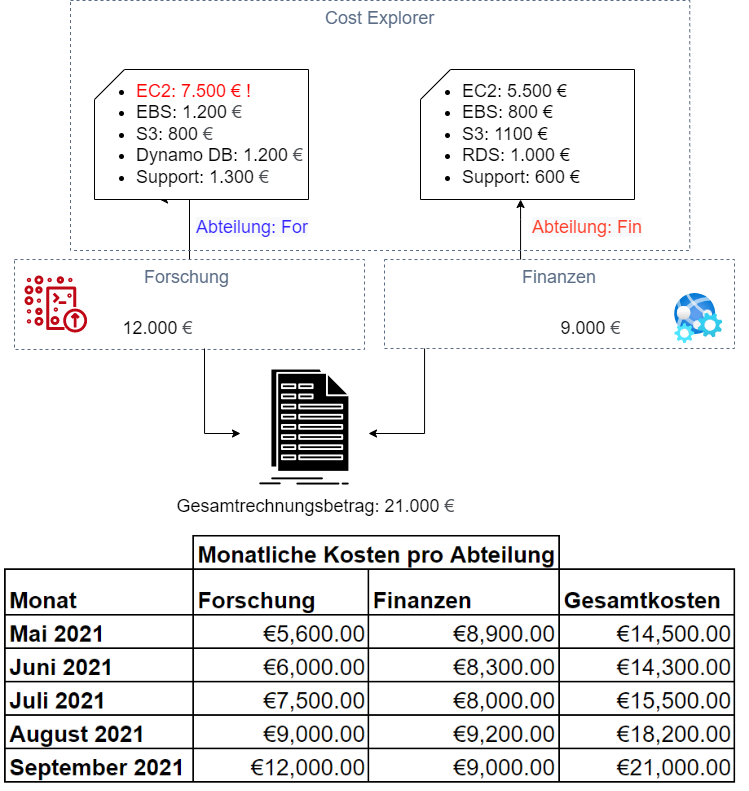
\includegraphics[scale=0.5]{sources/BA Diagramme-Nach Abteilung.drawio}
  \caption[Trennung der Kosten durch Tags]{}
  \label{fig:BA Diagramme-Nach Abteilung.drawio} 
  Trennung der Abteilungskosten durch Tags.\\
  Die Angaben dienen nur als Beispiel und entsprechen keiner realen IT-Infrastruktur.
  %\cite{AMZ20}
\end{figure} 
\\
In der \autoref{fig:BA Diagramme-Nach Abteilung.drawio} wird ein Szenario vorgestellt, wo die Kosten für EC2-Instanzen der Forschungsabteilung kontinuierlich angestiegen sind. Mitarbeiter der Forschungsabteilung waren nicht in der Lage, die Kostensteigerungen zu begründen. 
Um die von den einzelnen Abteilungen verursachten Kosten zu trennen, wurde ein Tag-Schlüssel mit dem Namen \textit{Abteilung} angelegt. Um anschließend jeder AWS-Dienst einen Tag-Wert entsprechend seiner Abteilung zuzuweisen. Mit Hilfe des Cost-Explorer konnte festgestellt werden, dass die Kosten für EC2 der Forschungsabteilung im Laufe der Zeit gestiegen sind. Nach Angaben der Abteilungsleiter hatte die Nutzung der Rechnerkapazität nicht zugenommen. Im vorliegenden Fall wurde festgestellt, dass Gastpraktikanten in der Forschungsabteilung Experimente durchführt, wo EC2-Instanzen genutzt haben. Die Instanzen wurden nach Beendigung des Aufenthalts nicht mehr abgeschaltet und haben kontinuierlich Kosten verursacht. 
\\\\
Für diesen hypothetischen Fall wurde die Ursache für den Anstieg der Gesamtkosten einer einfachen Organisation mit zwei Abteilungen und wenigen Cloud-Diensten ermittelt. Es gibt Unternehmen mit viel komplexeren Strukturen als diese, die weitaus mehr Cloud-Dienste in Anspruch nehmen. Für Unternehmen ist eine Tagging-Strategie von Relevanz, um Kosten für die Buchhaltungsabteilung zu ermittelt %internes Rechnungswesen
und um Budgets auf der Grundlage früherer Projekte erstellen zu können. Die Kostenüberwachung ist mit einer Tag-Strategie auf eine detaillierte Ebene möglich. Je nach festgelegten Tags können sehr detaillierte Analysen der Cloud-Nutzung und -Kosten über Produkte, Einheiten, Umgebungen oder beliebige andere Bereiche hinweg erstellt werden\footnote{\cite{CCB},Cloud Computing Basics: a Non.-Technical Introduction. Seite 152}.
%TRACK untagged services with a Budget.
%Si se quiere ser estricto con los costos de servicios que no tienen un Tag asignado se es posible rastrear estos costos creando un presupuesto filtrando servicios que no tienen un Tag asignado y crear una alarma si un umbral del presupuesto es sobrepasado.
%In den Best-Practices für Kostenüberwachung wird empfohlen, so bald wie möglich mit der Zuweisung von Tags zu Cloud-Diensten zu beginnen. QUELLE?
%Zu diesem Zweck werden Werkzeuge vorgestellt, die die Überwachung aktiver Diensten ermöglichen.
%Welche Kosten sind mit der Nutzung dieser Werkzeuge verbunden?
%Es sollte gezeigt werden, die Arten/Kategorien von Kunden, die kostenlosen Zugang zu diesen Werkzeuge haben?
%WAS MIT AWS Budgets? AWS Bill and cost Man.?
\subsection{AWS CloudWatch}
%https://aws.amazon.com/de/cloudwatch/pricing/
%https://docs.aws.amazon.com/AmazonCloudWatch/latest/monitoring/GettingStarted.html
Amazon CloudWatch ermöglicht die Überwachung der Leistung von Diensten, auch bei Diensten, die über verschiedene Regionen verteilt sind. CloudWatch sammelt operative Daten, welche zur Verlaufsanalyse und der Entscheidungsfindung in Bezug auf Optimierung und Fehlerbehebung hilfreicht sind. CloudWatch beschränkt sich nicht nur darauf, Daten aus der AWS-Umgebung zu empfangen. Externe Metriken, die mit CloudWatch kompatibel sind, können für eine einheitliche Analyse aggregiert werden. 
%El acceso a la informacion sobre los costos de los servicios actuales brinda lo necesario para que desiciones estrategicas puedan ser tomadas en base a numeros concretos. 
%Asi pueden diferentes departamentos de una organizacion sacar provecho y justificar sus desiciones (de compra). La transparencia sobre la informacion para tomar desiciones logra reducir el riesgo de la desicion. t.ly/cLGu S.27
%Wiki t.ly/9xO2
\\\\
Eine der Metriken zur Überwachung von EC2-Instanzen in CloudWatch ist die CPU-Auslastung oder CPU-Utilization auf Englisch. Basierend auf einem Prozentsatz der CPU-Auslastung können Benachrichtigungen und Aktionen konfiguriert werden. Eine dieser Aktionen ist die automatische Einrichtung neuer Instanzen zur Deckung des Kapazitätsbedarfs\footnote{\cite{AWS1},AWS Certified Solutions Architect - Associate (SAA-C02), Seite 185}. Diese Art von Aktionen werden im Kapitel ~\ref{kap_Optimierung} tiefer behandelt[ODER HIER?].
\\\\
Im Folgenden werden die grundlegenden Bereiche und Begriffe von CloudWatch erläutert und wie sie zur Überwachung von Informationen über AWS-Dienste verwendet werden.
\\\\
\textbf{Metriken} \\
Eine Metrik stellt eine Reihe von Daten über die Leistung eines Dienstes in zeitlicher Reihenfolge dar. Standardmäßig werden viele kostenlose Metriken an CloudWatch übermittelt.
\begin{comment}\\
Metriken bleiben wie folgt verfügbar:\\
Auflösung/Zeitraum: \\
1 Minute - 15 Tage\\
5 Minuten - 63 Tage.\\
1 Stunde - 15 Monate
\footnote{\cite{AMZ15}, Wie lange werden die verfügbaren Metriken aufbewahrt?}
\end{comment}
Zum Beispiel kann der Durchschnitt von einer bestimmten API pro Stunde untersucht werden. Für eine detailliertere Überwachung ist es möglich, benutzerdefinierte Metriken zu konfigurieren, die eine Auflösung von bis zu eine Sekunde zulassen. %Ein praktisches Beispiel für benutzerdefinierte Metriken ist die Messung der Ladezeit einer Website.
%[ANDERES BEISPIEL?]
% MIT BEZUG AUF K:OPTIMIERUNG?oder WIESO IST DIE AUFLÖSUNG RELEVANT?]
%\textbf{Logs} \\ BRAUCHE ICH DAS?
\\\\
\textbf{Ereignisse}\\
Ein Ereignis ist in CloudWatch eine Änderung in einem AWS Dienst. AWS-Dienste können Ereignisse erzeugen, wenn sich ihr Status ändert. %Das bedeutet, dass sich ein bestimmter AWS-Dienst selbst ändern kann. 
Beispielsweise, wird ein Ereignis erzeugt, wenn Amazon EC2 Auto Scaling, Instanzen gestartet oder beendet werden\footnote{\cite{AMZ13}, AWS Cloud Watch Events: User Guide. Seite 1} oder wenn eine bestimmte Menge an Speicherplatz in einem Bucket erreicht wurde. Ein Bucket ist ein Behälter, in dem Objekte bei Amazon S3 gespeichert werden\footnote{\cite{AMZ18}Amazon Simple Storage Service User Guide, Seite 4}. Beispiele für Objekte sind Dateien wie Bilder und Videos. 
\\\\
\textbf{Regel} \\
Eine Regel ordnet eintreffende Ereignisse zu und leitet diese zur Verarbeitung an Ziele weiter.
Eine einzelne Regel kann an mehrere Ziele weiterleiten, die alle parallel verarbeitet werden\footnote{\cite{AMZ13}, AWS Cloud Watch : User Guide. Seite 2}.
\\\\
\textbf{Ziele} \\
Ziele oder Targets sind AWS-Dienste, die aufgerufen werden, wenn eine Regel ausgelöst wird.
EC2 instances, AWS Lambda functions und Amazon SNS sind unter anderem mögliche Ziele.
Die Ziele einer Regel müssen sich in derselben Region wie die Regel befinden
\footnote{\cite{AMZ13}AWS Cloud Watch Events: User Guide. Seite 2}.
%Alle zugelassene AWS-Diensten \footnote\url{https://docs.aws.amazon.com/AmazonCloudWatch/latest/events/EventTypes.html}
\\\\
\textbf{Benachrichtigungen}\\
%https://docs.aws.amazon.com/AmazonCloudWatch/latest/monitoring/AlarmThatSendsEmail.html
Benachrichtigt zu werden ist wichtig, um relevante Ereignisse nicht zu verpassen und rechtzeitig Maßnahmen zu ergreifen. Mit CloudWatch können Alarme eingerichtet werden, die durch Metriken wie die CPU-Auslastung und Gebühren von einem spezifischen AWS-Dienst ausgelöst werden. Benachrichtigungen können durch Amazon SNS\footnote{\cite{AMZ30}Amazon SNS ist ein AWS-Dienst für die Benachrichtigung an Personen und an Applikationen.} oder zu einer E-Mail-Adresse geschickt werden.
Zu Testzwecken wurde ein Alarm erstellt, indem eine monatliche Ausgabengrenze von 9 Euro festgelegt wurde. Dieser ist in Anhang \ref{sec_Ang_B} zu finden.
%AUCH PER SLACK ODER ÄHNLICHES
%This could be a good example %https://youtu.be/__knpcBRLHg?t=770
%https://docs.aws.amazon.com/autoscaling/ec2/userguide/Cooldown.html
%Autoscaling group seted with cooldown periods to avoid too much instances to by launched.
%Most popular parts of CloudWatch:
%https://youtu.be/k7wuIrHU4UY?t=785
% LINKS :
%https://docs.aws.amazon.com/AmazonCloudWatch/latest/monitoring/GettingStarted.html
%https://docs.aws.amazon.com/AmazonCloudWatch/latest/monitoring/WhatIsCloudWatch.html
%https://docs.aws.amazon.com/AmazonCloudWatch/latest/monitoring/Install-CloudWatch-Agent.html
\subsubsection*{Visualisierung von Metriken}
Mit Cloud-Watch Dashboards können relevante Metriken grafisch dargestellt werden. %[BESSERE FORMULIERUNG] %Sie ermöglichen eine umfassende Visualisierung von Metriken der AWS-Diensten in der AWS-Umgebung. 
Durch die Dashboards können auch Benachrichtigungen erstellt werden. Für die Einrichtung der Benachrichtigungen ist kein technisches Wissen nötig\footnote{\cite{AMZ14}AWS Cloud Watch : User Guide. Seite 28}.
%Die von CloudWatch gesammelte Informationen sind nicht nur für System-Administratoren relevant.
Die in den Dashboards enthaltenen Informationen sind nicht nur für ihre Autoren von Relevanz. Weitere Personen innerhalb oder außerhalb einer Organisation können Zugriff auf Dashboards mit nützlichen Informationen bekommen, um Prozesse zu beschleunigen und Probleme schneller zu beheben. Um den Zugriff auf das Dashboard zu beschränken, ist es möglich, den Zugriff auf bestimmte Personen per E-Mail oder über SSO-Anmeldeinformationen\footnote{\cite{AMZ33} AWS Single Sign-On} zu beschränken. SSO (Single Sign-On) ist ein Prozess der einmaligen Authentifizierung und Zugriff auf mehrere Ressourcen. Ziel von SSO ist es, die Anzahl von von Login und Passwort in heterogenen Umgebungen zu reduzieren\footnote{\cite{SSO}Securing User Authentication using Single SignOn in Cloud Computing}. Außerdem hat die Einbindung von Dashboard-Informationen auf Infranet-Portale das Potenzial, Transparenz und eine schnelle Verbreitung von Informationen zu schaffen\footnote{\cite{BKM}Business Knowledge Management: Wertschöpfung durch Wissensportale.}. 
%Die Zugriffsverwaltung für geteilte Dashboards wird über AWS Identity and Access Management abgewickelt\footnote{\cite{AMZ14}AWS Cloud Watch : User Guide. Seite 18 und 39}[UND?].
\\\\
Zu Testzwecken wurde ein Dashboard mit einigen Widgets erstellt. Das erste Widget in der \autoref{fig:AWS_Trusted_Advisor_Kategorien} zeigt, wie oft auf die Objekte eines Buckets in S3 zugegriffen wird. Die andere zeigt die Anzahl der Aufrufe der CloudWatch-API an. Beide Widgets verwenden Standardmetriken, welche keine Kosten verursachen. Ein Widget ist ein grafischer Weg, um Metriken in CloudWatch darzustellen. Unter anderem gibt es Widgets für Zahlen, Linien, [More]etc.
[Rev update this]
\begin{figure}[h!]
  \centering
  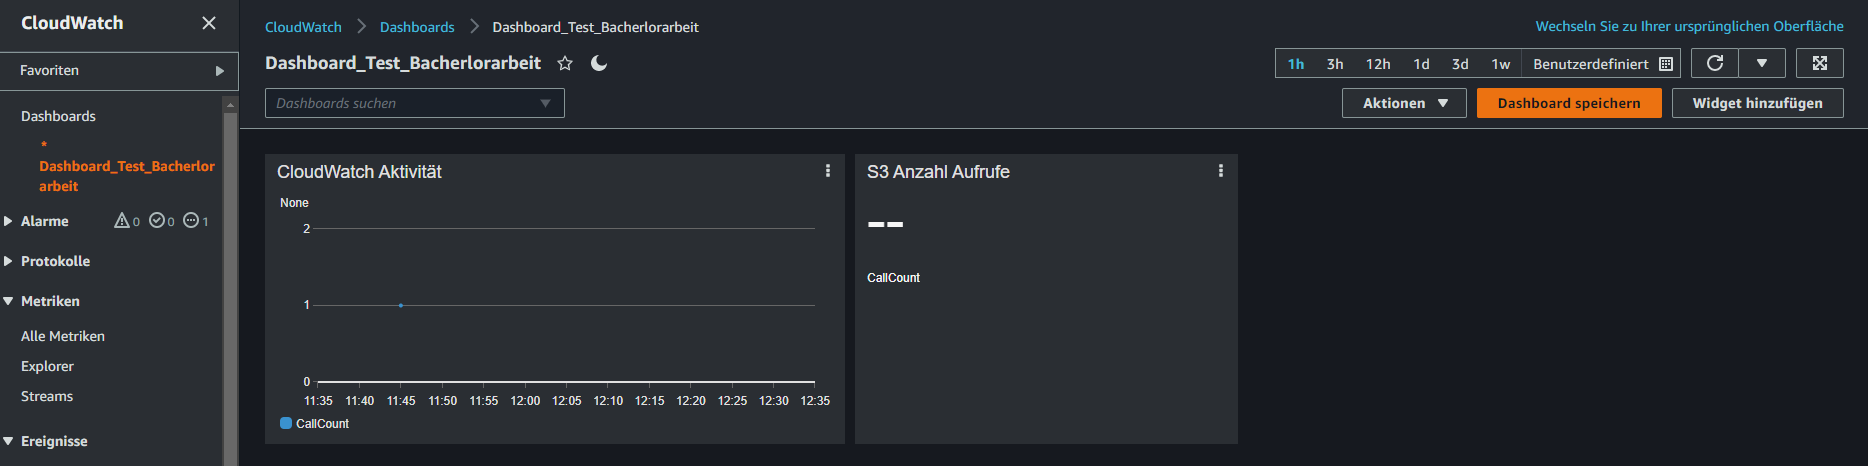
\includegraphics[scale=0.5]{sources/CloudWatchDashboardTest}
  \caption[Dashboard-Test in CloudWatch]{}
  \label{fig:CloudWatchDashboardTest} 
  Dashboard-Test in CloudWatch.
  %\cite{AMZ20}
\end{figure}
%t.ly/fNbyT
%https://cloudwatch.amazonaws.com/dashboard.html?dashboard=Dashboard_Bacherlorarbeit&context=eyJSIjoidXMtZWFzdC0xIiwiRCI6ImN3LWRiLTA0MzIyNjMwOTkwOCIsIlUiOiJ1cy1lYXN0LTFfTHdSdnczNE5CIiwiQyI6IjE2ZTdlb3VuajY1YTRhYjZsMjV2ZTZtY2pxIiwiSSI6InVzLWVhc3QtMTpmYzQ3OWYwNi1hYmNhLTQ1MzEtODRmZi0wNzYyMGVjYTBkNzciLCJNIjoiUHVibGljIn0=
Es wurde bereits erwähnt, dass es möglich ist, das Dashboard zu teilen, ohne Zugang zu Ihrem eigenen AWS-Konto gewähren zu müssen. Das hier erwähnte Dashboard wurde für den öffentlichen Zugriff temporär freigegeben. Über den Folgenden Link kann man auf das Dashboard zugreifen: \url{t.ly/fNbyT} \footnote{Falls der Link für das Dashboard abgelaufen ist, befindet sich ein Screenshot des Dashboards in Anhang \ref{sec_Ang_C}}. 


%t.ly/lRzA Establezca indicadores clave de rendimiento (KPI) ...
\subsubsection*{Fakturierungsalarme mit CloudWatch}
%Seite 145 Amazon CloudWatch - Benutzerhandbuch
AWS CloudWatch empfängt Abrechnungsmetriken von allen AWS-Diensten. Auch von AWS-Rechnungen, auf der Grundlage dieser Metriken ist es daher möglich, Regeln zu erstellen, die bei Überschreitung des geplanten Budgets Alarmen in Form von Benachrichtigungen auslösen.
Wenn ein bestimmter Prozentsatz oder Betrag des festgelegten Budgets überschritten wurde. Die oben genannten Alarme finden ihre Anwendung unter anderem im Kostenverlaufsplan. Der Kostenverlaufsplan gehört zum Projektmanagement, welcher Kosten eines Projekts phasenweise oder kumuliert bereitstellt\footnote{\cite{PM1}Kompakte Einführung in das Projektmanagement. Seite 96.}. Im Anhang \ref{sec_Ang_A} befindet sich die Vorlage für die Erstellung eines Fakturierungsalarms in JSON und YAML Format.
%\subsubsection*{Benachrichtigung bei Hoch- und Runterfahren von EC2-Instanzen}
%Obwohl Auto-Scaling dafür sorgt, die Rechenkapazität dynamisch anzupassen, ist es von größter Wichtigkeit, über Änderungen in der Infrastruktur informiert zu sein, ohne die Dashboards manuell überprüfen zu müssen.
%[WEIL .... LÖSCHEN?]
%\\\\
\subsection{AWS Cost-Explorer}\label{ssec:Cost-Explorer}
Cost-Explorer erstellt Berichte über die Kosten und die Nutzung von AWS-Diensten. Darüber hinaus wird eine Kostenprognose für die nächsten Monate erstellt, welche auf die Kosten der vergangenen Monaten basiert. Die Nutzung des Cost-Explorers ist kostenlos, nur API-Aufrufe sind kostenpflichtig \footnote{{\cite{AMZ22}AWS Cost Management Pricing}}.
%Mio:%Conocer clos costos en un periodo de tiempo nos permite %saber si estamos en el camino correcto para alcanzar las %metas trazadas al inicio del periodo/proyecto y tomar %las medidas adecuadas para que al final del periodo/%proyecto tengamos resultados satisfactorios.
\subsubsection*{Standardberichte}
Standardberichte sind vorgefertigte Berichte, die die Nutzung oder die Kosten nach einer selbstdefinierten Zeitraum zeigen. Diese zeigen eine grafische Darstellung der stündlichen, täglichen oder monatliche Kosten nach Dienst, die Abdeckung und die Auslastung von reservierten Instanzen oder die in Saving Plans Zahlungsmodell und die Ausgaben auf dem AWS Marketplace\footnote{{\cite{AMZ34}AWS Marketplace ist ein Einkaufskatalog für Software von Drittanbietern.}}. Die Berichte über die Abdeckung und Auslastung der reservierten Instanzen wurde im TrueCar-Anwendungsfall verwendet. Dies findet sich in Unterkapitel \ref{ssec:UseCaseTrueCar}.
\\\\
Eine weitere Verwendung dieser Informationen findet sich im Bereich der Marketing. Als Beispiel, ein Unternehmen, das ein Freemium-Dienst\footnote{\cite{MAR2}Ein Freemium-Dienst bietet in der Regel zwei Versionen an, eine kostenlose und eine kostenpflichtige.} anbietet. Die Marketingabteilung möchte eine Werbekampagne durchführen. Durch eine Werbekampagne werden in der Regel neue Nutzer generiert, und zwar sowohl zahlende als auch nicht zahlende Nutzer. Normalerweise gilt: Je mehr Nutzer, desto größer die Belastung für die IT-Infrastruktur. Um die im Zusammenhang mit der Werbekampagne durch neue Nutzer entstehenden Kosten zu messen, werden die tatsächlichen Kundenakquisitionskosten (CAC)\footnote{\cite{MAR1}Kundenakquisitionskosten sind alle anfallenden Kosten in der Customer Acquisition-Phase für ein Unternehmen.} berechnet, wobei nur die Kosten der nicht zahlenden Nutzer berücksichtigt werden. Zur Unterscheidung zwischen alten(vor der Werbekampagne) und neuen Nutzern wird das Datum der Erstellung des Nutzerkontos verwendet. Kunden, die aufgrund der Werbekampagne von der kostenlosen zur kostenpflichtigen Version des Dienstes gewechselt haben, werden in einer anderen Kategorie\footnote{{MAR3}Cost-per-Action (CPA)} ausgeschlossen.
%, die den Dienst nutzen, aber nicht dafür bezahlen. 
\\\\ 
Die Formel für die Berechnung der Kundenakquisitionskosten lautet wie folgt:\\
Anfallende Marketingkosten (MK) plus Vertriebskosten (VK) durch die Anzahl der gewonnenen Kunden (GK).\\
Kosten von Nutzern, die den Dienst kostenlos in Anspruch nehmen, würden in diesem Fall in den Vertriebskosten enthalten sein. Auf diese Weise ist die Marketingabteilung in der Lage, die tatsächlichen Kosten pro zahlenden Neukunden zu berechnen, die durch die Werbekampagne generiert wurden.  

\subsubsection*{Leistungskennzahlen (KPI)[Rev][Rev]}
Cost-Explorer-Berichte enthalten Daten, die die Merkmale eines guten KPI erfüllen. Sie sind spezifisch und in Bezug auf die Zeit messbar.
\\\\
In der \autoref{fig:Dashboard_EC2_S3} werden %das monatliche Geschäftswachstum, [Gelöscht, weil hier nicht relevant]
die durchschnittlichen Kosten pro Stunde für EC2-Instanzen, den Prozentsatz der Instanzen einer bestimmten Generation und der Vorgängerversionen, die Abdeckung nach Zahlungsmodell und die Verteilung des S3-Speichers nach Speicherklassen berechnet. Die oben genannten Metriken sammelt sichIn diesem Beispiel werden Metriken aus CloudWatch? und Informationen aus Cost-Explorer-Berichten zusammengestellt.
\begin{figure}[h!]
  \centering
  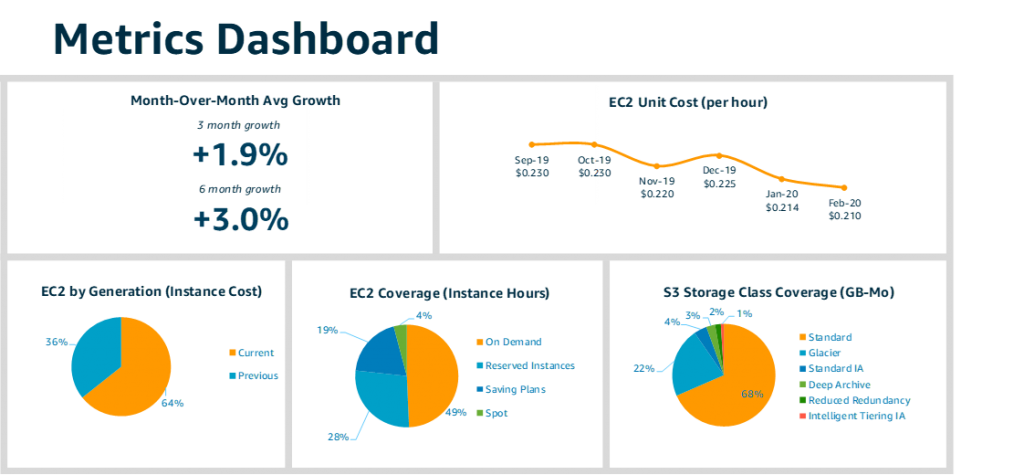
\includegraphics[scale=0.65]{sources/Dashboard_EC2_S3}
  \caption[Dashboard mit EC2 und S3 Metriken]{}
  \label{fig:Dashboard_EC2_S3} 
  Dashboard mit EC2 und S3 Metriken\cite{AMZ35}
\end{figure}\\
Die obengenannten Metriken stammen von CloudWatch. Wie in der \autoref{fig:OpsAnDiensteCloudWatch} zu sehen, ist es möglich, mathematische Operationen mit den Metriken durchzuführen, um zum Beispiel Durchschnittswerte, Prozentsätze und vieles mehr zu berechnen.
\begin{figure}[h!]
  \centering
  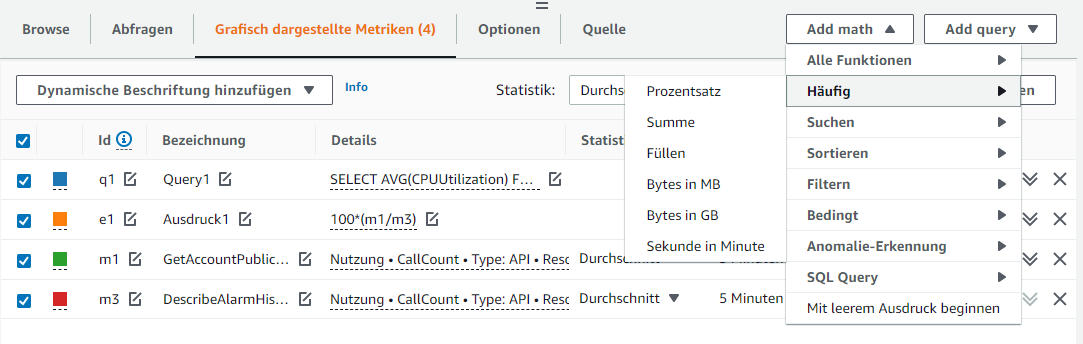
\includegraphics[scale=0.55]{sources/OpsAnDiensteCloudWatch}
  \caption[Operationen an Cloud-Diensten in CloudWatch]{}
  \label{fig:OpsAnDiensteCloudWatch} 
  Mathematische Operationen an Cloud-Diensten in CloudWatch.\\
  Quelle: CloudWatch AWS-Console
\end{figure}
%https://andrewchen.com/how-to-actually-calculate-cac/
%Sample KPIs: EC2 hourly or daily costs
%Value: Understand the EC2 unit cost per subscriber
%Sample KPIs: Cost by purchase option, purchase option coverage
%Value: Optimize your cost savings by leveraging pricing models
%Auslastungsbericht UND Abdeckungsbericht
%\subsubsection*{Berichte von reservierten Instanzen und Saving Plans}
[WAS DAMIT?]AWS analysiert die bisherige Nutzung der Instanzen und gibt Empfehlungen zur Kostensenkung durch den Wechsel von EC2-Instanzen in On-Demand Zahlungsmodell zu reservierten Instanzen. Diese ignorieren Kapazität, die bereits von anderen reservierten Instanzen abgedeckt wurden.
Es besteht die Möglichkeit, einen Bericht über die Nutzung von AWS-Diensten der letzten zwölf Monate einzusehen und zu prüfen, ob die Empfehlungen des Cost-Explorers angemessen sind.

\subsubsection*{Budgetplanung}
Die Budgetplanung ist eine Methode der Kostenkontrolle, die beim Start eines neuen Projekts eingesetzt wird\footnote{\cite{BUD2}Cost Control Methods: Definitions and Examples}. Der Bericht über die in den letzten zwölf Monaten entstandenen Kosten zusammen mit der Prognose der Kosten der kommenden zwölf Monaten[Rev] tragen zu einen guten Budgetplanung bei.
%%t.ly/6bvZ% https://youtu.be/3peNAKB3VxA?t=223
Durch die Möglichkeit, die in den letzten Monaten angefallenen Kosten nach bestimmten AWS-Diensten, Projekt oder Abteilung zu trennen, ist es möglich, operative Budgetplanungen aus vergangenen Projekten mit Genauigkeit zu erstellen. 
\begin{quote}
  „Bei der operativen Planung wird von einem Zeithorizont von einem Jahr ausgegangen. Hier liegt der Fokus darauf, Ressourcen konkret zuzuweisen und detailreicher zu planen. Welche Mittel werden wofür verwendet und welche kurz- und mittelfristigen Ziele sollen durch diesen Mitteleinsatz erreicht werden”\cite{BUD1}.
  In dem Fall dieser Arbeit sind die obengenannten Ressourcen die AWS-Dienste.
\end{quote}
Cost-Explorer liefert Informationen zur Rechtfertigung von Ausgaben aus im Voraus festgelegten Budgets, hilft bei der Planung künftiger Budgets und unterstützt die Verfolgung von KPIs.
%\textbf{Aktuelle Budgets vs erwartet=Soll-Ist-Vergleich Methode}
%Einer der Standardberichte im AWS Cost Explorer enthält die Kosten in Dollar/Euro und die Nutzung von EC2-Instanzen in Stunden pro Monat. Mit diesen Informationen können Sie die Kosten für eine bestimmte Dienstleistung berechnen. 
\subsection{AWS Trusted Advisor[Rev]}
%https://www.youtube.com/watch?v=i0IkKN9NoPk
%https://aws.amazon.com/de/premiumsupport/technology/trusted-advisor/
%Kunden von AWS Basic Support und AWS Developer Support können auf grundlegende Sicherheitsprüfungen und alle Prüfungen für Servicekontingente zugreifen. Kunden von AWS Business Support und AWS Enterprise Support können auf alle Prüfungen zugreifen, einschließlich Kostenoptimierung, Sicherheit, Fehlertoleranz, Leistung und Servicekontingente. 
%was macht dieses?
%AWS Trusted Advisor: This helps you know more about idle or underutilized resources.
AWS Trusted Advisor ist ein Werkzeug, das Empfehlungen zur Kostenreduzierung, Verbesserung der Systemverfügbarkeit und Erhöhung der Systemsicherheit gibt. Die Empfehlungen basieren auf Best-Practices, die im Laufe der Jahre durch die Beteuerung von AWS-Kunden gesammelt wurden und Prüfungen, die auf dem bestehenden AWS-Konto durchgeführt wurden.
In dieser Arbeit werden Empfehlungen in Bezug auf Servicekontingente und Kostenoptimierung insbesondere betrachtet, weil es sich um Empfehlungen handelt, die mit Kostenüberwachung und -optimierung zusammenhängen. Der Status von Prüfungen von Trusted Advisor sind über CloudWatch Events zugänglich. 

Es ist zu berücksichtigen, dass nur limitierte Sicherheitsprüfungen (6 Prüfungen Stand November 2021) für Konten in den Plänen Developer und Basic Support kostenlos sind. Prüfungen für die Kategorie Servicekontingente sind kostenlos. Detaillierte Informationen und Empfehlungen von der Kategorien Kostenoptimierung, Performance und Fehlertoleranz sind nur zugänglich, wenn ein Business- oder Enterprise-Konto vorliegt\footnote{\cite{AMZ36}Trusted Advisor}. \\
%ES MUSS GEPRÜFT WERDEN, OB ES SINNVOLL IST, FÜR DIE OBEN GENANNTEN SUPPORT-PLÄNEN ZU ZAHLEN.
\begin{figure}[h!]
      \centering
      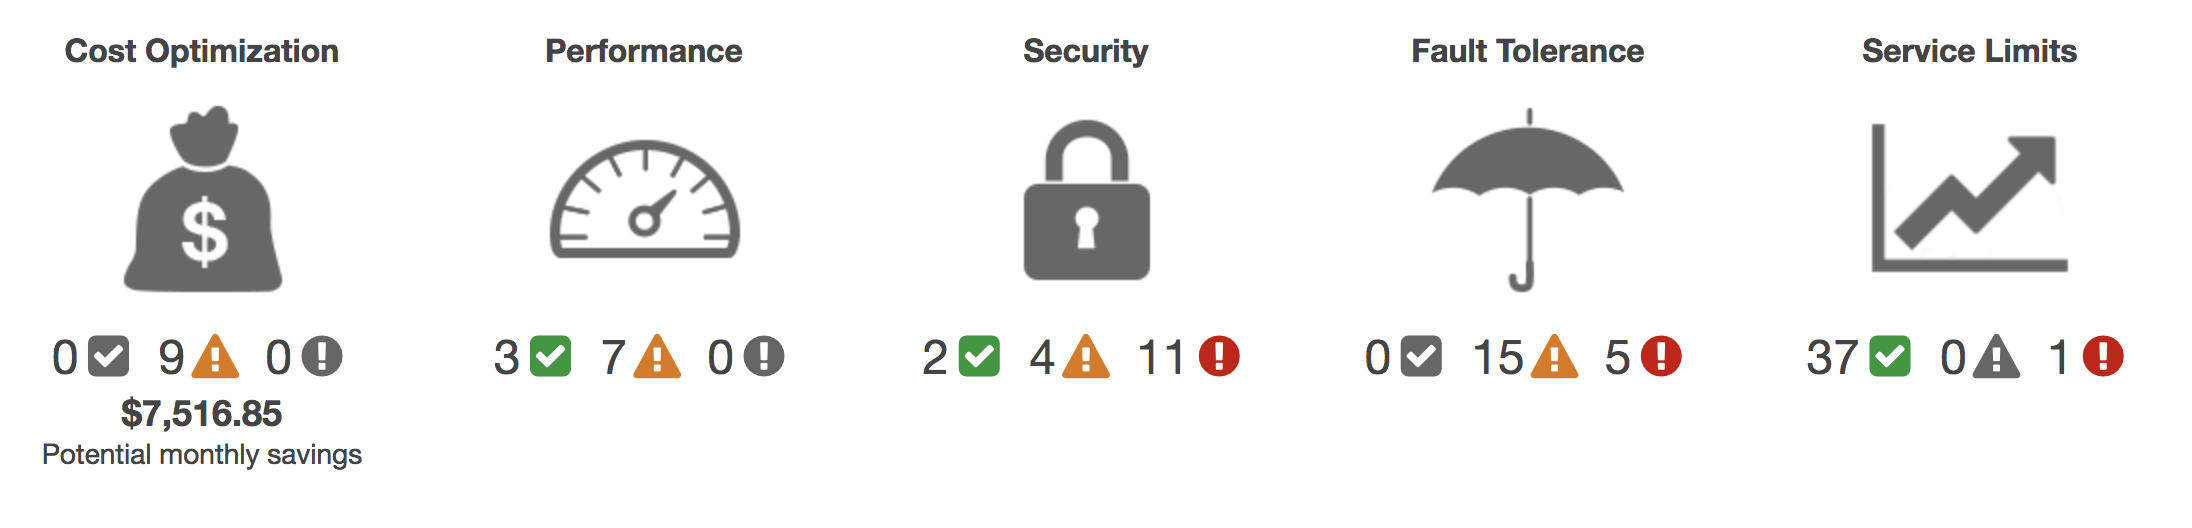
\includegraphics[scale=0.4]{sources/AWS_Trusted_Advisor_Kategorien}
      \caption[AWS Trusted Advisor Kategorien]{}
      \label{fig:AWS_Trusted_Advisor_Kategorien} 
      AWS Trusted Advisor Kategorien\cite{AMZ20}
\end{figure}
Die \autoref{fig:AWS_Trusted_Advisor_Kategorien} zeigt die fünf Kategorien von Trusted Advisor mit jeweils 3 Arten von Indikatoren. Die Indikatoren zeigen an, welche Prüfungen durchgeführt wurden. Grün bedeutet, dass keine Fehler oder zu prüfenden Empfehlungen vorhanden sind. Warnungen werden durch orangefarbene Indikatoren und Fehler durch rote Indikatoren angezeigt. Diese Empfehlungen sind eine Zusammenfassung auf hohem Niveau. Sie sind ein Startpunkt für die Untersuchung von AWS-Diensten mit Hilfe anderer Werkzeuge wie CloudWatch oder Cost-Explorer.%[ODER?].
\\\\

\subsection*{Kategorie Kostenoptimierung}
Die Empfehlungen zur Kostenoptimierung konzentrieren sich auf Möglichkeiten zur Kostensenkung, indem ungenutzte AWS-Diensten hervorgehoben werden. 
%[BEISPIELE]
\subsubsection*{EC2}
Sollten EC2-Instanzen mit geringer Auslastung gefunden werden, wird es diese bei Trusted Advisor signalisiert. Denn diese Instanzen verbrauchen verursachen Kosten und können terminiert oder pausiert werden. %[HIER FEHLT...]
Auch nicht zugewiesene Elastic IP-Adressen(EIP) erzeugen Kosten. Diese können gegebenenfalls von Trusted Advisor gefunden werden. EIPs maskieren den Ausfall einer Instanz oder Availability Zone, indem eine öffentliche IP-Adresse einer anderen Instanz oder Availability Zone neu zugewiesen wird\footnote{\cite{AMZ37}AWS Support - Benutzerhandbuch. Seite 65.}. %t.ly/nYiv


\subsubsection*{Kategorie Servicekontingente}
In dieser Kategorie werden Empfehlungen zur Vermeidung von Grenzwertüberschreitungen hervorgehoben.
Es wird zum Beispiel nach einer Nutzung gesucht, die mehr als 80 \% des Leistungsgrenzwerten für wichtige Dienste beträgt. Einige Beispiele sind  Amazon EC2, Auto Scaling, Elastic Block Store, Simple Email Service und AWS CloudFormation.
\\\\
Sich dieser Grenzen bewusst zu sein, gibt die Möglichkeit, rechtzeitig zu handeln und es trägt zu Kostenüberwachung bei.
[GLEICHE GRENZEN WIE BEI CloudWatch?]

\subsubsection*{Trusted-Advisor Kosten/Erwägungen}
Bei der Erwägung von Trusted-Advisor ist zu überlegen, ob es kosteneffizient ist, für Support-Pläne zu zahlen, die den Zugang zu allen Empfehlungen des Trusted Advisors ermöglichen. Eines der Ziele dieser Arbeit ist es, die Entstehung der Kosten auf eine praktikable Weise zu verstehen (Kostenüberwachung). %Dies, um Optimierungsmaßnahmen zu ermöglichen. 
\\
Es wäre nicht sinnvoll, Kosten für AWS-Dienste wie Geschäfts- oder Enterprise Support zu übernehmen, wenn diese die möglichen Einsparungen übersteigen. Die Vorteile von Geschäfts- oder Enterprise Support-Plänen beschränken sich nicht auf Kosteneinsparungen und Kostenbegrenzung, sondern tragen auch zur Sicherheit und Leistung bei. Jedes Unternehmen muss selbst entscheiden, ob es diese Informationen benötigt.
[ZEIGE BEISPIELE FueR Empfehlungen][Hier die Handlungen?]
\\   
\subsection{Überwachungswerkzeuge gemäß ihrer Verwendung}
Die \autoref{fig:ÜberwachungswerkzeugeNachVerwendung} fasst die Überwachungswerkzeuge zusammen und listet die Verwendung der einzelnen Werkzeuge auf.
\begin{figure}[h!]
  \centering
  \includegraphics[scale=0.6]{sources/ÜberwachungswerkzeugeNachVerwendung}
  \caption[Überwachungswerkzeuge gemäß ihrer Verwendung]{}
  \label{fig:ÜberwachungswerkzeugeNachVerwendung} 
  Überwachungswerkzeuge gemäß ihrer Verwendung\\
  Eigene Darstellung\cite{AMZ12, AMZ20, AMZ21}. 
\end{figure}
[NOCH NICHT VOLLSTÄNDIG]


\subsection*{Fazit}
 % CloudWatch
In diesem Kapitel wurde gezeigt, dass es mit CloudWatch möglich ist, Alarme auf Basis von Ereignissen einzurichten, die mit Amazon SNS oder externen E-Mail-Adressen kommunizieren. %Im nächsten Kapitel wird CloudWatch erneut behandelt. Diesmal nicht als Überwachungswerkzeug, sondern als Optimierungswerkzeug zur Erstellung von automatisierte Aktionen/Reaktionen. 
%Dazu war es notwendig, die Rolle der von CloudWatch gesammelten Metriken zu verstehen, die die Grundlage für die Verwaltung von Aktionen wie Auto-Scaling-Gruppen bilden. 
%Cost Explorer
Aus dem Blickwinkel des Kostenmanagements wurde gezeigt, dass mit Cost-Explorer eine Analyse von Kosten der letzten 12 Monate, eine Einschätzung der Kosten im aktuellen Monat und eine Prognose für die nächsten Monate möglich ist. Diese Informationen dient unter anderem zur Erstellung einer operativen Budgetplanung mit genaueren Daten, da
Kosten nach Tags und anderen Filtern getrennt werden können.
%Trusted Advisor
Darüber hinaus wurde Trusted Advisor vorgestellt, die konkrete Optimierungsempfehlungen gibt und warnt über Leistungsgrenzen. Dies kann mit erheblichen Kosten verbunden sein und ist daher nicht für alle Arten von Unternehmen unmittelbar attraktiv. Obwohl sich nicht alle Unternehmen die Prüfungen von Trusted Advisor leisten können, sollten die kostenlosen Empfehlungen im Überwachungs- und Optimierungsplan berücksichtigt werden.
[WAS KOMMT IN NÄCHTEN KAP.?]

\begin{comment}
En este capitulo se  mostró de qué manera es posible con CloudWatch configurar alarmas basadas en eventos. Dichas alarmas comunican con Amazon SNS o direcciones de correo externas. En el capiulo siguiente se volverá a tematizar CloudWatch. Esta vez no como herramienta de monitoneo, sino de optimizacion para crear acciones ??? Para ello fue necesario entender que papel juegan las metricas recolectadas por CloudWatch, las cuales son la base para manejar los grupos Auto-Scaling. 

Desde la perspectiva del manejo de costos, se mostró como con Cost-Explorer es posible analizar los costos de los ultimos 12 meses, tener un calculo de los costos en el mes actual y recibir un pronostico de los proximos meses. Teniendo la posibilidad de separar los costos por medio de Tags y otros filtros. Dicha información contribuye a poder crear una planificacion de presupuestos operativa basada en datos de gran presicion.

Además se presentaron herramientas como Trusted Advisor las cuales brindan recomendaciones concretas sobre optimizacion y alertan si limites que se acercan a su umbral máximo. 

Este puede representar costos consideradable y que por lo tanto no lo hacen directamente atractivo para todo tipo de empresas.
\end{comment}

\begin{comment}
AWS Cost-Explorer Budgets show actual spend vs budget by month.
Filter by budgets, tags and tax, region, instances, usage type, cost category
Die Kosten vorhersehbar machen
Wiederverwendung gespeicherter Berichte. Welche Vorteile?

Da kann man sehen wie viele Stunden an RI und an On-Demand pro Tag/Monat verbraucht wurden.
-	Informationen um Schätzungen handelt, die von den tatsächlichen Kosten für den Abrechnungszeitraum abweichen können. %https://youtu.be/3peNAKB3VxA?t=705
-	Kann ich die Usage von S3 Einheiten und analysieren, wie häufig diese zugegriffen werden %https://youtu.be/pjrKDkzbas8?t=2425
-	Man könnte herausfinden, ob die RIs tatsächlich günstiger als ON-Demand sind. Wenn die RIs sind „konvertierbar“ und teurer als On-Demand, könnte man sich dafür entscheiden diese in was umzuwandeln, was genutzt wird. %https://youtu.be/pjrKDkzbas8?t=3385

%(How to use Spots and on-demand)
%detect CPU Utilization, with Amazon CloudWatch
\end{comment}
%I could compute the cost of a query, user, transaction
